
\documentclass{beamer}
%\beamertemplateshadingbackground{brown!70}{yellow!10}
\mode<presentation>
{
  %\usetheme{Warsaw}
  \usecolortheme{crane}
  % or ...

%  \setbeamercovered{transparent}
  % or whatever (possibly just delete it)
}
\setbeamertemplate{navigation symbols}{}
%\setbeamertemplate{footline}[frame number]{}
\usepackage{tikz,pgfplots}
\pgfplotsset{compat=newest}
\usepackage[utf8]{inputenc}
\usetikzlibrary{patterns}
\usepackage{amssymb}
\usepackage{amsmath}
\usepackage{colortbl}
%\usepackage{multicol}
\usepackage{cancel}
\usepackage{ulem}
\usepackage{multirow}
\usepackage{relsize}
\usepackage{algorithm}
\usepackage{algorithmic}
\usepackage{forloop}% http://ctan.org/pkg/forloop
\newcounter{loopcntr}
\newcommand{\rpt}[2][1]{%
  \forloop{loopcntr}{0}{\value{loopcntr}<#1}{#2}%
}
%\pagestyle{plain}
%\input{defs2}
\def\opt{{\textsc{OPT}_k}}
\def\const{{\mathrm{const}}}
\def\nnz{{\mathrm{nnz}}}
\def\r{\sfrac{\sigma_{\w}^2}{\sigma_{\xib}^2}}
\def\rm{\sfrac{\sigma_{\xib}^2}{\sigma_{\w}^2}}
\def\cmark{\Green{\checkmark}}
\def\xmark{\Red{\large\sffamily x}}
\newcommand{\pdet}{{\mathrm{pdet}}}
\newcommand{\MSPE}[1] {{\mathrm{MSPE}\big[#1\big]}}
\newcommand{\MSE}[1] {{\mathrm{MSE}\big[#1\big]}}
\def\Poisson{{\operatorname{Poisson}}}
\def\PB{{\operatorname{PB}}}
\newcommand{\DP}[1]{\mathcal{DP}^{#1}}
\def\Ic{\mathcal{I}}
\def\Jc{\mathcal{J}}
\def\Mc{\mathcal M}
\def\Ec{\mathcal E}
\def\sr{{\mathrm{sr}}}
\def\ktd{{k^{\underline{d}}}}
\def\Det{{\mathrm{Det}}}
\def\detu{{\widecheck{\mathrm{Det}}_\mu^\gamma}}
\def\deto{{\widehat{\mathrm{Det}}_\mu^\gamma}}
\def\Zu{{\widecheck{Z}_\mu^{\gamma}}}
\def\Zo{{\widehat{Z}_\mu^{\gamma}}}
\def\Zun{{\widecheck{Z}_\mu^{\gamma_n}}}
\def\Zon{{\widehat{Z}_\mu^{\gamma_n}}}
\newcommand{\Er}{\mathrm{Er}}
\newif\ifDRAFT
\DRAFTtrue
\ifDRAFT
\newcommand{\marrow}{\marginpar[\hfill$\longrightarrow$]{$\longleftarrow$}}
\newcommand{\niceremark}[3]
   {\textcolor{red}{\textsc{#1 #2:} \marrow\textsf{#3}}}
\newcommand{\ken}[2][says]{\niceremark{Ken}{#1}{#2}}
\newcommand{\manfred}[2][says]{\niceremark{Manfred}{#1}{#2}}
\newcommand{\michael}[2][says]{\niceremark{Michael}{#1}{#2}}
\newcommand{\michal}[2][says]{\niceremark{Michal}{#1}{#2}}
\newcommand{\feynman}[2][says]{\niceremark{Feynman}{#1}{#2}}
%\usepackage[inline]{showlabels}
\else
\newcommand{\ken}[1]{}
\newcommand{\michael}[1]{}
\newcommand{\michal}[1]{}
\newcommand{\feynman}[1]{}
\fi
\newcommand{\norm}[1]{{\| #1 \|}}

\newcommand{\deff}{d_{\textnormal{eff}}}
\def\ee{\mathrm{e}}
\newcommand\mydots{\makebox[1em][c]{.\hfil.\hfil.}}
\def\Sd{\mathscr{S}_{\!d}}
\newcommand{\dx}{\dxy_{\!\cal X}}
\newcommand{\dxk}{\dxy_{\!\cal X}^k}
\newcommand{\dk}{\dxy^k}
\newcommand{\dxy}{\mathrm{D}}
\def\simiid{\overset{\textnormal{\fontsize{6}{6}\selectfont
i.i.d.}}{\sim}}
%\newcommand{\Dxy}{D_{\!\cal X\!,\cal Y}}
\def\vskx{{\mathrm{VS}_{\!\dx}^k}}
\def\vsk{{\mathrm{VS}_{\!D}^k}}
\def\vskxm{{\mathrm{VS}_{\!\dx}^{k-1}}}
\def\vskm{{\mathrm{VS}_{\!D}^{k-1}}}
\def\vsdx{{\mathrm{VS}_{\!\dx}^d}}
\def\vsd{{\mathrm{VS}_{\!D}^d}}
\newcommand{\vs}[1]{{\mathrm{VS}_{\!D}^{#1}}}
\newcommand{\sigd}{\boldsymbol\Sigma_{\!\dx}}
\def\wols{\w_{\mathrm{LS}}}
\def\wds{\boldsymbol\w_{\!D}^*}
\def\kd{K_{\!\dx}}

\def\poly{{\mathrm{poly}}}
\def\polylog{{\mathrm{polylog}}}
\def\DPP{{\mathrm{DPP}}}
\def\DPPcor{{\DPP_{\!\mathrm{cor}}}}
\def\DPPens{{\DPP_{\!\mathrm{ens}}}}
\newcommand{\DPPreg}[1]{{\DPP_{\!\mathrm{reg}}^{#1}}}
\def\Vol{{\mathrm{VS}}}
\def\Lev{{\mathrm{Lev}}}
\newcommand\todod[1]{\Red{\# DH: #1}}
\newcommand{\explain}[2]{\mathrel{\overset{\makebox[0pt]{\text{\tiny
#1}}}{#2}}}
\def\tot {{\mathrm{tot}}}
\def\checkmark{\tikz\fill[scale=0.4](0,.35) -- (.25,0) --
(1,.7) -- (.25,.15) -- cycle;}
\newcommand{\mnote}[1]{{\bf\large \Magenta{*}}\marginpar{\small \Magenta{#1}}}
\newcommand{\bnote}[1]{{\bf #1}}

\newcommand{\sqrtshort}[1]{{\sqrt{\white{\Big|}\!\!\smash{\text{\fontsize{9}{9}\selectfont$#1$}}}}}
\newenvironment{proofof}[2]{\par\vspace{2mm}\noindent\textbf{Proof of {#1} {#2}}\ }{\hfill\BlackBox}
\newcommand{\sets}[2]
{{\hspace{-0.3mm}[\hspace{-0.3mm}#1\hspace{-0.3mm}]\hspace{-0.3mm}\choose
\hspace{-0.3mm}#2\hspace{-0.3mm}}}
\DeclareMathOperator{\sgn}{\textnormal{sgn}}
\DeclareMathOperator{\adj}{\textnormal{adj}}
\def\Rb{{\mathbf{R}}}
\DeclareMathOperator{\ws}{\widetilde{\w}}
\newcommand{\inote}[1]{{\bf {#1}}}
\def\xib{\boldsymbol\xi}
\def\Sigmab{\mathbf{\Sigma}}
\def\Sigmabh{\widehat{\Sigmab}}
\def\Sigmabt{\widetilde{\Sigmab}}
\def\S{\mathbf{S}}
\def\T{\mathbf{T}}
\def\xt{\tilde{x}}
\def\xbt{\widetilde{\x}}
\def\xbh{\widehat{\x}}
\def\ubh{\widehat{\u}}
\def\dom {{\mathrm{dom}}}
\def\val {{\mathrm{val}}}
\def\out {{\mathrm{out}}}
\def\iin  {{\mathrm{iin}}}
\def\s {\mathbf{s}}
\def\q {\mathbf{q}}
\def\qt{\tilde{q}}
\def\itld {j}
\def\ubt {\tilde{\u}}
\def\n{\{1..n\}}
\def\cb {\mathbf{c}}
\def\cW{\mathcal W}
\def\Xt{\widetilde{X}}
\def\Dbt{\widetilde{\D}}
\def\xtb{\tilde{\mathbf{x}}}
\def\ytb{\tilde{\mathbf{y}}}
\def\Xtb{\widetilde{\mathbf{X}}}
\def\Xbb{\overline{\X}}
\def\Xb{{\bar{\X}}}
\def\ybb{\overline{\y}}
\def\f{{\mathbf{f}}}
\def\g{{\mathbf{g}}}
\def\fbb{{\overline{\f}}}
\def\fb{{\overline{f}}}
\def\Xc{\mathcal{X}}
\def\W{\mathbf W}
\def\L{\mathbf{L}}
\def\Rb{\mathbf R}
\def\Pc{\mathcal{P}}
\def\Nc{\mathcal{N}}
\def\Pt{\widetilde{P}}
\def\Hc{\mathcal{H}}
\def\Wc{\mathcal{W}}
\def\Cc{\mathcal{C}}
\def\p{\mathbf p}
%\def\r{\mathbf r}
\def\Y{\mathbf Y}
\def\H{\mathbf H}
\def\K{\mathbf K}
\def\Kh{\widehat{K}}
\def\Kbh{{\widehat{\K}}}
\def\Q{\mathbf Q}
\def\Qbar{{\bar{\mathbf Q}}}
\def\Ytb{\widetilde{\mathbf{Y}}}
\def\c{{n-d\choose s-d}}
\DeclareMathOperator{\Proj}{Proj}
\newcommand{\Span}{\mathrm{span}}
\newcommand{\ofsubt}[1]{\mbox{\scriptsize \raisebox{0.25pt}{$(#1)$}}}
%\raisebox{0.5pt}{$($}}#1\mbox{\tiny \raisebox{0.5pt}{$)$}}}
\newcommand{\ofsub}[1]{\mbox{\small \raisebox{0.0pt}{$(#1)$}}}
%\newcommand{\ofsubb}[1]{\mbox{\footnotesize \raisebox{0.5pt}{$(#1)$}}}
%\newcommand{\ofsub}[1]{(#1)}
%\newcommand{\ofsub}[1]{\mbox{\tiny$|$\hspace{-0.5pt}\raisebox{-0.5pt}{$#1$}}}
\newcommand{\of}[2]{{#1{\!\ofsub{#2}}}}
\newcommand{\oft}[2]{{#1{\!\ofsubt{#2}}}}
\newcommand{\fof}[2]{{#1({#2})}}
\newcommand{\yof}[2]{{#1{\ofsub{#2}}}}
%\newcommand{\yofb}[2]{{#1{\ofsubb{#2}}}}
\newcommand{\lazy}{FastRegVol}
\newcommand{\volsamp}{RegVol}

\newcommand{\Sm}{{S_{-i}}}
\newcommand{\Sp}{{S_{+i}}}
\ifx\BlackBox\undefined
\newcommand{\BlackBox}{\rule{1.5ex}{1.5ex}}  % end of proof
\fi
%\renewcommand{\dagger}{+}
\DeclareMathOperator*{\argmin}{\mathop{\mathrm{argmin}}}
\DeclareMathOperator*{\argmax}{\mathop{\mathrm{argmax}}}
\DeclareMathOperator*{\diag}{\mathop{\mathrm{diag}}}
\def\x{\mathbf x}
\def\y{\mathbf y}
\def\ybh{\widehat{\mathbf y}}
\def\ybb{\bar{\mathbf y}}
\def\xbb{\bar{\mathbf x}}
\def\yb{{\bar y}}
\def\ybt{\widetilde{\mathbf y}}
\def\yh{\widehat{y}}
\def\yhb{\widehat{\y}}
\def\yt{\widetilde{y}}
\def\z{\mathbf z}
\def\a{\mathbf a}
\def\b{\mathbf b}
\def\w{\mathbf w}
\def\v{\mathbf v}
\def\m{\mathbf m}
\def\wbh{\widehat{\mathbf w}}
\def\wh{\widehat{\mathbf w}}
\def\vbh{\widehat{\mathbf v}}
\def\wbt{\widetilde{\mathbf w}}
\def\e{\mathbf e}
\def\zero{\mathbf 0}
\def\one{\mathbf 1}
\def\u{\mathbf u}
\def\ubbar{\bar{\mathbf u}}
\def\f{\mathbf f}
\def\ellb{\boldsymbol\ell}

\def\X{\mathbf X}
\def\Xs{\widetilde{\X}}
\def\B{\mathbf B}
\def\A{\mathbf A}
\def\C{\mathbf C}
\def\U{\mathbf U}
\def\Ubt{\widetilde{\mathbf U}}
\def\Ubh{\widehat{\mathbf U}}
\def\Ubbar{\bar{\mathbf U}}
\def\F{\mathbf F}
\def\D{\mathbf D}
\def\V{\mathbf V}
\def\M{\mathbf M}
\def\Mh{\widehat{\mathbf M}}
%\def\S{\mathbf S}
\def\Stb{\widetilde{\mathbf{S}}}
\def\Sbh{\widehat{\mathbf{S}}}
\def\St{\widetilde{\S}}
\def\Sh{\widehat{S}}
\def\Sc{\mathcal{S}}
\def\Fc{\mathcal{F}}
\def\Vc{\mathcal{V}}
\def\Bc{\mathcal{B}}
\def\Dc{\mathcal{D}}
\def\Z{\mathbf Z}
\def\Zbh{\widehat{\mathbf Z}}
\def\Zbt{\widetilde{\mathbf Z}}
\def\Abh{\widehat{\mathbf A}}
\def\I{\mathbf I}
\def\Ic{\mathcal I}
\def\II{\mathbf {I \!\,I}}
%\def\II{\boldsymbol {\mathbb I}}
\def\A{\mathbf A}
\def\P{\mathbf P}
\def\Ph{\widehat{\mathbf P}}
\def\cP{\mathcal P}
\def\cR{\mathcal R}
\def\Xt{\widetilde{\mathbf{X}}}
\def\Xh{\widehat{\mathbf{X}}}
\def\Rh{\widehat{R}}
\def\Ot{\widetilde{O}}
\def\At{\widetilde{\A}}


\def\E{\mathbb E}
\def\R{\mathbb R}
\def\N{\mathbb N}
\def\Pr{\mathrm{Pr}}
%\def\C{\mathbb C}
\def\tr{\mathrm{tr}}
\def\Sbar{{\bar{S}}}
\def\cS{{\mathcal{S}}}
\def\Tbar{{\bar{T}}}
\def\Tt{{\widetilde{T}}}
\def\rank{\mathrm{rank}}
\def\Prob{\mathrm{Prob}}
\def\Var{\mathrm{Var}}
\def\Xinv{(\X^\top\X)^{-1}}
\def\XinvS{(\X_S\X_S^\top)^{-1}}
\def\ABinvS{(\A_S\B_S^\top)^{-1}}
\def\ABinv{(\A\B^\top)^{-1}}
\def\xinv{\x_i^\top\Xinv\x_i}
\def\Xinvr{(\lambda\I+\X_{-1}^\top\X_{-1})^{-1}}
\def\pdet{\mathrm{pdet}}
\newcommand{\vol}{\mathrm{vol}}
%\newcommand{\defeq}{:=}
\newcommand{\defeq}{\stackrel{\textit{\tiny{def}}}{=}}
\newcommand{\di}{{[d+1]_{-i}}}
\newcommand{\cov}{\mathrm{cov}}
\let\origtop\top
\renewcommand\top{{\scriptscriptstyle{\origtop}}} % this makes transpose not so big

\definecolor{silver}{cmyk}{0,0,0,0.3}
\definecolor{yellow}{cmyk}{0,0,0.9,0.0}
\definecolor{reddishyellow}{cmyk}{0,0.22,1.0,0.0}
\definecolor{black}{cmyk}{0,0,0.0,1.0}
\definecolor{darkYellow}{cmyk}{0.2,0.4,1.0,0}
\definecolor{orange}{cmyk}{0.0,0.7,0.9,0}
\definecolor{darkSilver}{cmyk}{0,0,0,0.1}
\definecolor{grey}{cmyk}{0,0,0,0.5}
\definecolor{darkgreen}{cmyk}{0.6,0,0.8,0}
\newcommand{\Red}[1]{{\color{red}  {#1}}}
\newcommand{\Purple}[1]{{\color{purple}  {#1}}}
\newcommand{\Magenta}[1]{{\color{magenta}{#1}}}
\newcommand{\Green}[1]{{\color{darkgreen}  {#1}}}
\newcommand{\Blue}[1]{\color{blue}{#1}\color{black}}
\newcommand{\Orange}[1]{\textcolor{orange}{#1}\color{black}}
\newcommand{\Brown}[1]{{\color{brown}{#1}\color{black}}}
\newcommand{\Grey}[1]{{\color{grey}{#1}\color{black}}}
\newcommand{\white}[1]{{\textcolor{white}{#1}}}
\newcommand{\yellow}[1]{{\textcolor{reddishyellow}{#1}}}
\newcommand{\darkYellow}[1]{{\textcolor{darkYellow}{#1}}}
\newcommand{\grey}[1]{{\textcolor{grey}{#1}}}

\DeclareMathOperator{\half}{\frac{1}{2}}

\ifx\proof\undefined
\newenvironment{proof}{\par\noindent{\bf Proof\ }}{\hfill\BlackBox\\[2mm]}
\fi

\ifx\theorem\undefined
\newtheorem{theorem}{Theorem}
\fi

\ifx\example\undefined
\newtheorem{example}{Example}
\fi

\ifx\condition\undefined
\newtheorem{condition}{Condition}
\fi
\ifx\property\undefined
\newtheorem{property}{Property}
\fi

\ifx\lemma\undefined
\newtheorem{lemma}{Lemma}
\fi

\ifx\proposition\undefined
\newtheorem{proposition}{Proposition}
\fi

\ifx\remark\undefined
\newtheorem{remark}{Remark}
\fi

\ifx\corollary\undefined
\newtheorem{corollary}{Corollary}
\fi

\ifx\definition\undefined
\newtheorem{definition}{Definition}
\fi

\ifx\conjecture\undefined
\newtheorem{conjecture}{Conjecture}
\fi

\ifx\axiom\undefined
\newtheorem{axiom}{Axiom}
\fi

\ifx\claim\undefined
\newtheorem{claim}{Claim}
\fi

\ifx\assumption\undefined
\newtheorem{assumption}{Assumption}
\fi

\ifx\condition\undefined
\newtheorem{condition}{Condition}
\fi


\edef\polishl{\l}
\setlength{\columnsep}{0.7em}
\setlength{\columnseprule}{0mm}
\setlength{\arrayrulewidth}{1pt} 

\newcommand{\svr}[1]{{\textcolor{darkSilver}{#1}}}
\definecolor{brightyellow}{cmyk}{0,0,0.7,0.0}
\definecolor{lightyellow}{cmyk}{0,0,0.3,0.0}
\definecolor{lighteryellow}{cmyk}{0,0,0.1,0.0}
\definecolor{lightestyellow}{cmyk}{0,0,0.05,0.0}
\AtBeginSection[]
{
\begin{frame}<beamer>
\frametitle{Outline}
\tableofcontents[currentsection]
\end{frame}
}


%  \fboxsep=3pt
% %\fboxsep=0mm%padding thickness
% \fboxrule=2pt%border thickness


\setkeys{Gin}{width=0.7\textwidth}

\title[]{Minimax experimental design:\\
\small Bridging the gap between statistical and worst-case approaches to least squares regression}

\author[]{\small \hspace{-0.2cm}Micha{\l} Derezi\'{n}ski, Ken Clarkson, Michael Mahoney,
  Manfred Warmuth\\
 ~\quad 
\includegraphics[width=0.1\textwidth]{../sty/Berkeley.png}\qquad\qquad
  
\includegraphics[width=0.09\textwidth]{../sty/IBM.png}\qquad\quad\quad
\includegraphics[width=0.1\textwidth]{../sty/Berkeley.png}\qquad\quad
\includegraphics[width=0.125\textwidth,viewport=0 160 375 261,clip]{../sty/UCSC}~
\includegraphics[width=0.09\textwidth] {../sty/Google.jpg}}
% \author[]{$\text{
%   \begin{tabular}{c@{\qquad}c@{\qquad}c@{\qquad}c}
%   Micha{\polishl} Derezi\'{n}ski
%   & Kenneth L.~Clarkson
%   & Michael W.~Mahoney
%   & Manfred K.~Warmuth\end{tabular}}$}
%   \\[1mm]
% 
\includegraphics[height=1.5em]{../sty/Berkeley.png}
%   &
\includegraphics[height=1.5em]{../sty/IBM.png}
%   & 
\includegraphics[height=1.5em]{../sty/Berkeley.png}
%   & 
\includegraphics[height=1.5em,viewport=0 160 375 261,clip]{../sty/UCSC}
%       \hspace{1mm}
% 	
\includegraphics[height=1.5em] {../sty/Google.jpg}
% \end{tabular}
%}
\date{
  COLT'19\\
  June 27, 2019}

\begin{document}
\begin{frame}
  \titlepage
\end{frame}

\linespread{1.3}

\begin{frame}
  \frametitle{Classical experimental design}
  Consider $n$ parameterized experiments:
  $\x_1,\dots,\x_n\in\R^d$.\\
  Each experiment has a \underline{hidden} random response $y_i$ such that:
  \begin{align*}
    y_i = \x_i^\top\w^* + \xi_i,\qquad \xi_i\sim\Nc(0,\sigma^2)
  \end{align*}
  \pause
\textbf{Goal:} Select $k\ll n$ experiments to best estimate $\w^*$
  \pause
\begin{columns}
\begin{column}{0.3\textwidth}
\\ \vspace{0.8cm}
Select $S=\{4,6,9\}$\\
\vspace{1cm}
Receive $y_4, y_6, y_9$
\end{column}
\begin{column}{0.5\textwidth}
\begin{center}
	\begin{tikzpicture}[scale=0.9]
          \draw [fill=brown!30] (-2,0) rectangle (0,3);
          \draw [color=black] (-2,2) -- (0,2);
          \draw (-2.25,2) node {\mbox{\footnotesize $\x_4^\top$}}; 
          \draw [color=black] (-2,1.5) -- (0,1.5);
          \draw (-2.25,1.5) node {\mbox{\footnotesize $\x_6^\top$}}; 
          \draw [color=black] (-2,0.5) -- (0,0.5);
          \draw (-2.25,0.5) node {\mbox{\footnotesize $\x_9^\top$}}; 
	   \draw (-3,3) node {fixed $\X$}; 
           \draw [decorate,decoration={brace}] (-2,3.1) -- (0,3.1);
          \draw (-1,3.4) node {\mbox{\fontsize{8}{8}\selectfont $d$}}; 
            \draw [color=lightgray,line width =0.5mm] (1,0) -- (1,3);
            \draw [color=lightgray] (0.75,3) node {$\y$};
            \draw (0.75,2) node {\mbox{\footnotesize $y_4$}}; 
            \draw (1,2) node {.}; 
            \draw[mark=*,mark size=1.5pt] plot coordinates{(1,2)};
            \draw (0.75,1.5) node {\mbox{\footnotesize $y_6$}}; 
            \draw (1,1.5) node {.}; 
            \draw[mark=*,mark size=1.5pt] plot coordinates{(1,1.5)};
            \draw (0.75,0.5) node {\mbox{\footnotesize $y_9$}}; 
            \draw[mark=*,mark size=1.5pt] plot coordinates{(1,.5)};
	\end{tikzpicture}
\end{center}
\end{column}
\end{columns}

\end{frame}

\begin{frame}
  \frametitle{A-optimal design}
  Find an unbiased estimator $\wbh$ with smallest
  \textit{mean squared error}:
  \begin{align*}
\text{minimize}\quad
    \underbrace{\E_{\wbh}\big[\|\wbh-\w^*\|^2\big]}_{\mathrm{MSE}[\wbh]}\quad\text{subject
    to}\quad\E\big[\wbh\big]=\w^*\ \ \forall_{\w^*}
  \end{align*}
  \pause
Given every $y_1,\dots,y_n$, the optimum is \textit{least squares}: $\wbh=\X^\dagger\y$
  \begin{align*}
\MSE{\X^\dagger\y}=\tr\big(\Var[\X^\dagger\y]\big)=\sigma^2\underbrace{\tr\big((\X^\top\X)^{-1}\big)}_{\phi}
  \end{align*}
  \pause
  \vspace{-4mm}
  
% \begin{center}\fcolorbox{reddishyellow}{lightyellow}{
%   \parbox{0.95\textwidth}{
  \begin{theorem}[based on \cite{avron-boutsidis13}]
   There is an experimental design $S$ of size
$k\leq\Blue{d+\phi/\epsilon}$ such that
$$\mathrm{MSE}[\X_S^\dagger\y_S]\leq \epsilon\cdot
\underbrace{\tr(\Var[\xib])}_{n\sigma^2}$$
\vspace{-2mm}
% }}\end{center}
\end{theorem}
\pause
\Red{
    Required assumption:\quad $y_i = \x_i^\top\w^* +
    \xi_i,\quad\xi_i\sim\Nc(0,\sigma^2)$
  }
\end{frame}

\begin{frame}
  \frametitle{What if $\xi_i$ is not $\Nc(0,\sigma^2)$?}
  \begin{align*}
    \y&\text{ - any random vector in $\R^n$ with finite second moment}
    \\
\onslide<2->{    \w^*_{\y|\X}&\defeq  \argmin_\w \E_\y \big[\|\X\w-\y\|^2\big]
}
    \\ \onslide<3->{\xib_{\y|\X}&\defeq \y-\X\w_{\y|\X}^*
\quad\text{- deviation from best linear predictor}}
  \end{align*}
  \pause\pause\pause\vspace{3mm}

Two special cases:\vspace{2mm}
\pause
\begin{enumerate}
\item Statistical regression:\quad\quad\
  $\E\big[\xib_{\y|\X}\big]=\zero$\quad (mean-zero noise)
  \pause
\item Worst-case regression:\quad $\Var\big[\xib_{\y|\X}\big]=\zero$ \quad
  (deterministic $\y$)
\end{enumerate}

\end{frame}

\begin{frame}
  \frametitle{Random experimental designs}
  \textbf{Statistical:}  \ \,Fixed $S$ is ok\\
  \textbf{Worst-case:} Fixed $S$ can be exploited by the
  adversary\pause
  \vspace{5mm}
  
\begin{definition}
We define a \underline{random experimental design} $(S,\wbh)$
of size $k$ as:
  \begin{enumerate}
    \item a random subset $S\subseteq \{1..n\}$ s.t.~$|S|\leq k$
    \item a jointly random function $\wbh:\R^{|S|}\rightarrow\R^d$
    \end{enumerate}
    \end{definition}
    \vspace{6mm}
    
% $\Wc_k(\X)$ - family of \textit{unbiased} random experimental designs
% $(S,\wbh)$ of size $k$:
%     \begin{align*}
%       \E_{S,\wbh,\y}\big[\wbh(\y_S)\big] = \w^*_{\y|\X}
%       \qquad \text{for all }\y\in\Fc_n
%     \end{align*}
\end{frame}

  \begin{frame}
    \frametitle{Experimental design with arbitrary responses}
    \begin{theorem}[main result]
For any $\epsilon>0$, there is a random experimental design $(S,\wbh)$
of size
\[k=O(\Blue{d}\,\Red{\log n}\Blue{\,+\,\phi/\epsilon}), \quad\text{where}\quad\phi=\tr\big((\X^\top\X)^{-1}\big),\]
such that for any random $\y$ we have
\begin{align*}
\text{(unbiasedness)}\quad  \E\big[\wbh(\y_S)\big]&= \w^*_{\y|\X},\\[3mm]
\mathrm{MSE}\big[\wbh(\y_S)\big] - \mathrm{MSE}\big[\X^\dagger\y\big]
  &\leq \epsilon\cdot 
  \E\big[\|\xib_{\y|\X}\|^2\big]%\quad\text{and}\quad k= O(d\log n + \phi/\epsilon).
\end{align*}
\end{theorem}
% \pause\vspace{4mm}

% \textit{Toy example:} \quad$\Var[\xib_{\y|\X}]=\sigma^2\I$,\quad\ 
% $\E[\xib_{\y|\X}]=\zero$
% \pause\vspace{3mm}
% \begin{enumerate}
%   \item $\E\big[\|\xib_{\y|\X}\|^2\big]
%     %\tr\big(\Var[\xib_{\y|\X}]\big) + \big\|\E[\xib_{\y|\X}]\big\|^2
%     =\tr\big(\Var[\xib_{\y|\X}]\big)$
%     \pause\vspace{1mm}
%   \item $\MSE{\X^\dagger\y} %= \sigma^2\phi    %\leq \sigma^2k\epsilon\ll
%     % \sigma^2n \epsilon
%     = \frac\phi n\cdot \tr\big(\Var[\xib_{\y|\X}]\big)$
%   \end{enumerate}
  % \pause\vspace{3mm}
  
  % So in this case $\mathrm{MSE}\big[\wbh(\y_S)\big]\leq
  % O(\epsilon) \cdot \tr\big(\Var[\xib_{\y|\X}]\big)$ as expected
\end{frame}

\begin{frame}
  \frametitle{Important special instances}
  \begin{enumerate}
  \item    \textit{Statistical regression:}\quad
    $\y = \X\w^*+\xib$,\quad $\E[\xib]=\zero$
    % \begin{align*}
    %   \mathrm{MSE}\big[\wbh(\y_S)\big] -
    %   \mathrm{MSE}\big[\X^\dagger\y\big]\leq \epsilon\cdot\tr\big(\Var[\xib]\big)
    % \end{align*}
    \pause\vspace{2mm}
    \begin{itemize}
    \item Weighted regression:\quad\ 
      $\Var[\xib]=\mathrm{diag}\big([\sigma_1^2,\dots,\sigma_n^2]\big)$\\[2mm]
      \pause
      \item Generalized regression: $\Var[\xib]$ is
        arbitrary
        % \pause
        % \item Bayesian regression: \quad \,$\w^*\sim\Nc(\zero,\I)$
        \end{itemize}
        \pause\vspace{5mm}
      \item \textit{Worst-case regression:}\quad $\y$ is any fixed vector in
        $\R^n$
%         \pause
%         \begin{align*}
%       \E_{S,\wbh}\big[\|\wbh(\y_S)-\w^*\|^2\big]\leq \epsilon\cdot
%           \|\y-\X\w^*\|^2
%         \end{align*}
% where $\w^*=\X^\dagger\y$
  \end{enumerate}
\end{frame}

\begin{frame}
  \frametitle{Main result: proof outline}
  \pause
  \begin{enumerate}
  \item Unbiased estimators via volume sampling\\[4mm]\pause
  \item Error bounds via i.i.d.~importance sampling:\\[1mm]\pause
    \begin{enumerate}
    \item Leverage score sampling:\quad  $\Pr(i) \defeq \frac1d \x_i^\top(\X^\top\X)^{-1}\x_i$\\[1mm]\pause
    \item Inverse score sampling:\quad \ \,$\Pr(i)\defeq
     \frac1\phi\x_i^\top(\X^\top\X)^{-2}\x_i$\quad\Red{(new)}
    \end{enumerate}
  \end{enumerate}
\end{frame}


\begin{frame}
\frametitle{Volume sampling}
  \begin{definition}
  Given a  full rank matrix  $\X\in\R^{n\times d}$ we define volume sampling
  $\Vol(\X)$ as a distribution over sets $S\subseteq [n]$ of size $d$:
  \vspace{-1mm}
  \begin{align*}
    \Pr(S) =
    \frac{\det(\X_S)^2}{\det(\X^\top\X)}.
  \end{align*}
\end{definition}\pause
\begin{columns}
  \begin{column}{0.59\textwidth}
$$
\Pr(S)\sim \!\!{\footnotesize
\begin{array}{l}
  \text{squared volume}\\
  \text{of the parallelepiped} \\
\text{spanned by $\{\x_i:i\!\in\! S\}$}
\end{array}
}
$$
{\footnotesize Computational cost: $O(\mathrm{nnz}(\X)\log n+d^4\log d)$}
\end{column}
\begin{column}{.35\textwidth}
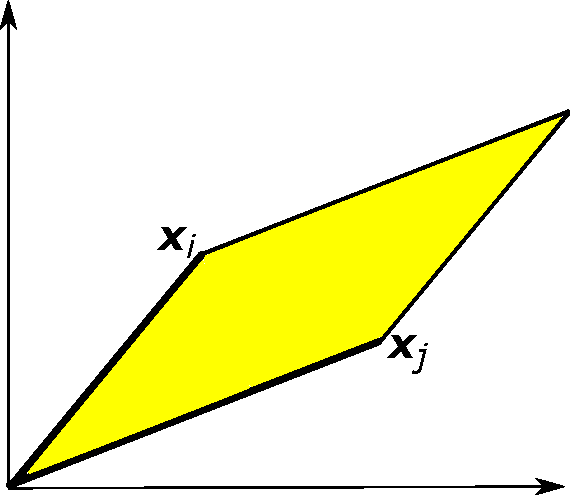
\includegraphics[width=\textwidth]{../talk/figs/volume_simple}
\end{column}
\end{columns}
\end{frame}

\begin{frame}
  \frametitle{Unbiased estimators via volume sampling}
  Under arbitrary response model, any i.i.d.~sampling is \underline{biased}
\begin{theorem}[\cite{correcting-bias}]
Volume sampling corrects the least squares bias of i.i.d.~sampling.
\end{theorem}\pause
\vspace{3mm}
Let $q=(q_1,\dots,q_n)$ be some i.i.d.~importance sampling.
\begin{align*}
\text{\footnotesize volume + i.i.d.}\quad
  &\overbrace{\x_{i_1},\mydots,\x_{i_d}}^{\sim\Vol(\X)},\
  \overbrace{\x_{i_{d+1}},\,\x_{i_{d+2}},\mydots,\,\x_{i_{k}}}^{\sim q^{k-d}}
\end{align*}
\pause
\begin{align*}
  \E\bigg[\argmin_\w\sum_{t=1}^k\frac1{q_{i_t}}(\x_{i_t}^\top\w-y_{i_t})^2\bigg]
  = \w_{\y|\X}^*
\end{align*}
\end{frame}

% \begin{frame}
%   \frametitle{Importance sampling for experimental design}
%   \begin{enumerate}
%   \item  \textit{Leverage score sampling}: $\Pr(i)=p_i^{\mathrm{lev}}
% \defeq \frac1d \x_i^\top(\X^\top\X)^{-1}\x_i$\\
% {\footnotesize A standard sampling method for worst-case linear regression.}
% \pause
% \vspace{5mm}

%   \item \textit{Inverse score sampling}: $\Pr(i)= p_i^{\mathrm{inv}}\defeq
%     \frac1\phi\x_i^\top(\X^\top\X)^{-2}\x_i$.\\
% {\footnotesize  A novel sampling technique essential
%     for achieving $O(\phi/\epsilon)$ sample size.}
%   \end{enumerate}
% \end{frame}

\begin{frame}
  \frametitle{Conclusions}

  \begin{enumerate}
  \item Experimental design with \underline{arbitrary responses}
    \pause
  \item Upper bound almost matches the Gaussian noise setting
  \end{enumerate}  \pause
  \textbf{Open problems:}
  \begin{enumerate}
  \item Eliminating the $\Red{\log n}$ factor
  \item Efficiently finding \underline{minimax} optimal designs:
  \end{enumerate}
  \begin{definition}
    Minimax optimal experimental design with unbiased estimators:
\begin{align*}
R_k^*(\X)&\defeq 
  \min_{(S,\wbh)}\ \max_{\y}\,\frac{\mathrm{MSE}\big[\wbh(\y_S)\big]-
     \mathrm{MSE}\big[\X^\dagger\y\big]
  }{\E\big[\|\xib_{\y|\X}\|^2\big]}
\end{align*}
\end{definition}
\end{frame}

\begin{frame}
  \frametitle{References}
  \footnotesize
\bibliographystyle{alpha}
\bibliography{../pap}
\end{frame}

\end{document}